% How the global random state takes part when a function draws in the body of
% nv_while(), which runs a number of times not known when it is traced: the
% function; the graph jit() traces from it, with the part that implements the
% random state in blue and its unused part in gray; the views of the random
% state in the program's trace and in the body's; the host object; and
% numbered notes on what happens.
% Build: see figures/README.md
\documentclass[tikz, border = 6pt]{standalone}
\usepackage[T1]{fontenc}
\usepackage{lmodern}
\usetikzlibrary{positioning, calc, fit, backgrounds, matrix}

\definecolor{keep}{HTML}{2A7AB0}

% The part of the graph that implements the side effect, and the part of it
% that is not used.
\newcommand{\se}[1]{\textcolor{keep}{#1}}
\newcommand{\unused}[1]{\textcolor{black!40}{#1}}
% An annotation next to a line of the graph.
\newcommand{\aside}[1]{\hspace{1.5em}{\normalfont\sffamily\itshape\color{black!60}$\leftarrow$ #1}}
\newcommand{\cd}[1]{\texttt{#1}}

\tikzset{
  badge/.style = {circle, fill = black!65, text = white, font = \sffamily\tiny\bfseries,
    inner sep = 0pt, minimum size = 3.2mm, anchor = base},
  lines/.style = {matrix of nodes, row sep = {3.9mm, between origins}, column sep = 2pt,
    nodes = {anchor = base west, inner sep = 0.5pt, font = \ttfamily\scriptsize},
    column 2/.style = {nodes = {badge}}, column 3/.style = {nodes = {badge}}},
  fields/.style = {matrix of nodes, row sep = {3.9mm, between origins}, column sep = 2pt,
    nodes = {anchor = base west, inner sep = 0.5pt, font = \ttfamily\scriptsize},
    column 1/.style = {nodes = {text = black!55}}},
  box/.style = {rounded corners = 2pt, inner sep = 5pt},
  head/.style = {font = \footnotesize\bfseries, text = black!70, anchor = south west,
    inner sep = 1pt},
  note/.style = {font = \footnotesize, align = left, text width = 8.6cm, anchor = north west,
    inner sep = 0pt, execute at begin node = {\thickmuskip = 5mu}}
}

% A note: its text at #2, numbered #1 in a badge hanging to its left.
\newcommand{\note}[3]{
  \node[note] (#1) at #2 {#3};
  \node[badge, font = \sffamily\scriptsize\bfseries, minimum size = 3.8mm, anchor = north east]
    at ($(#1.north west) + (-0.15, 0.04)$) {#1};
}

\begin{document}
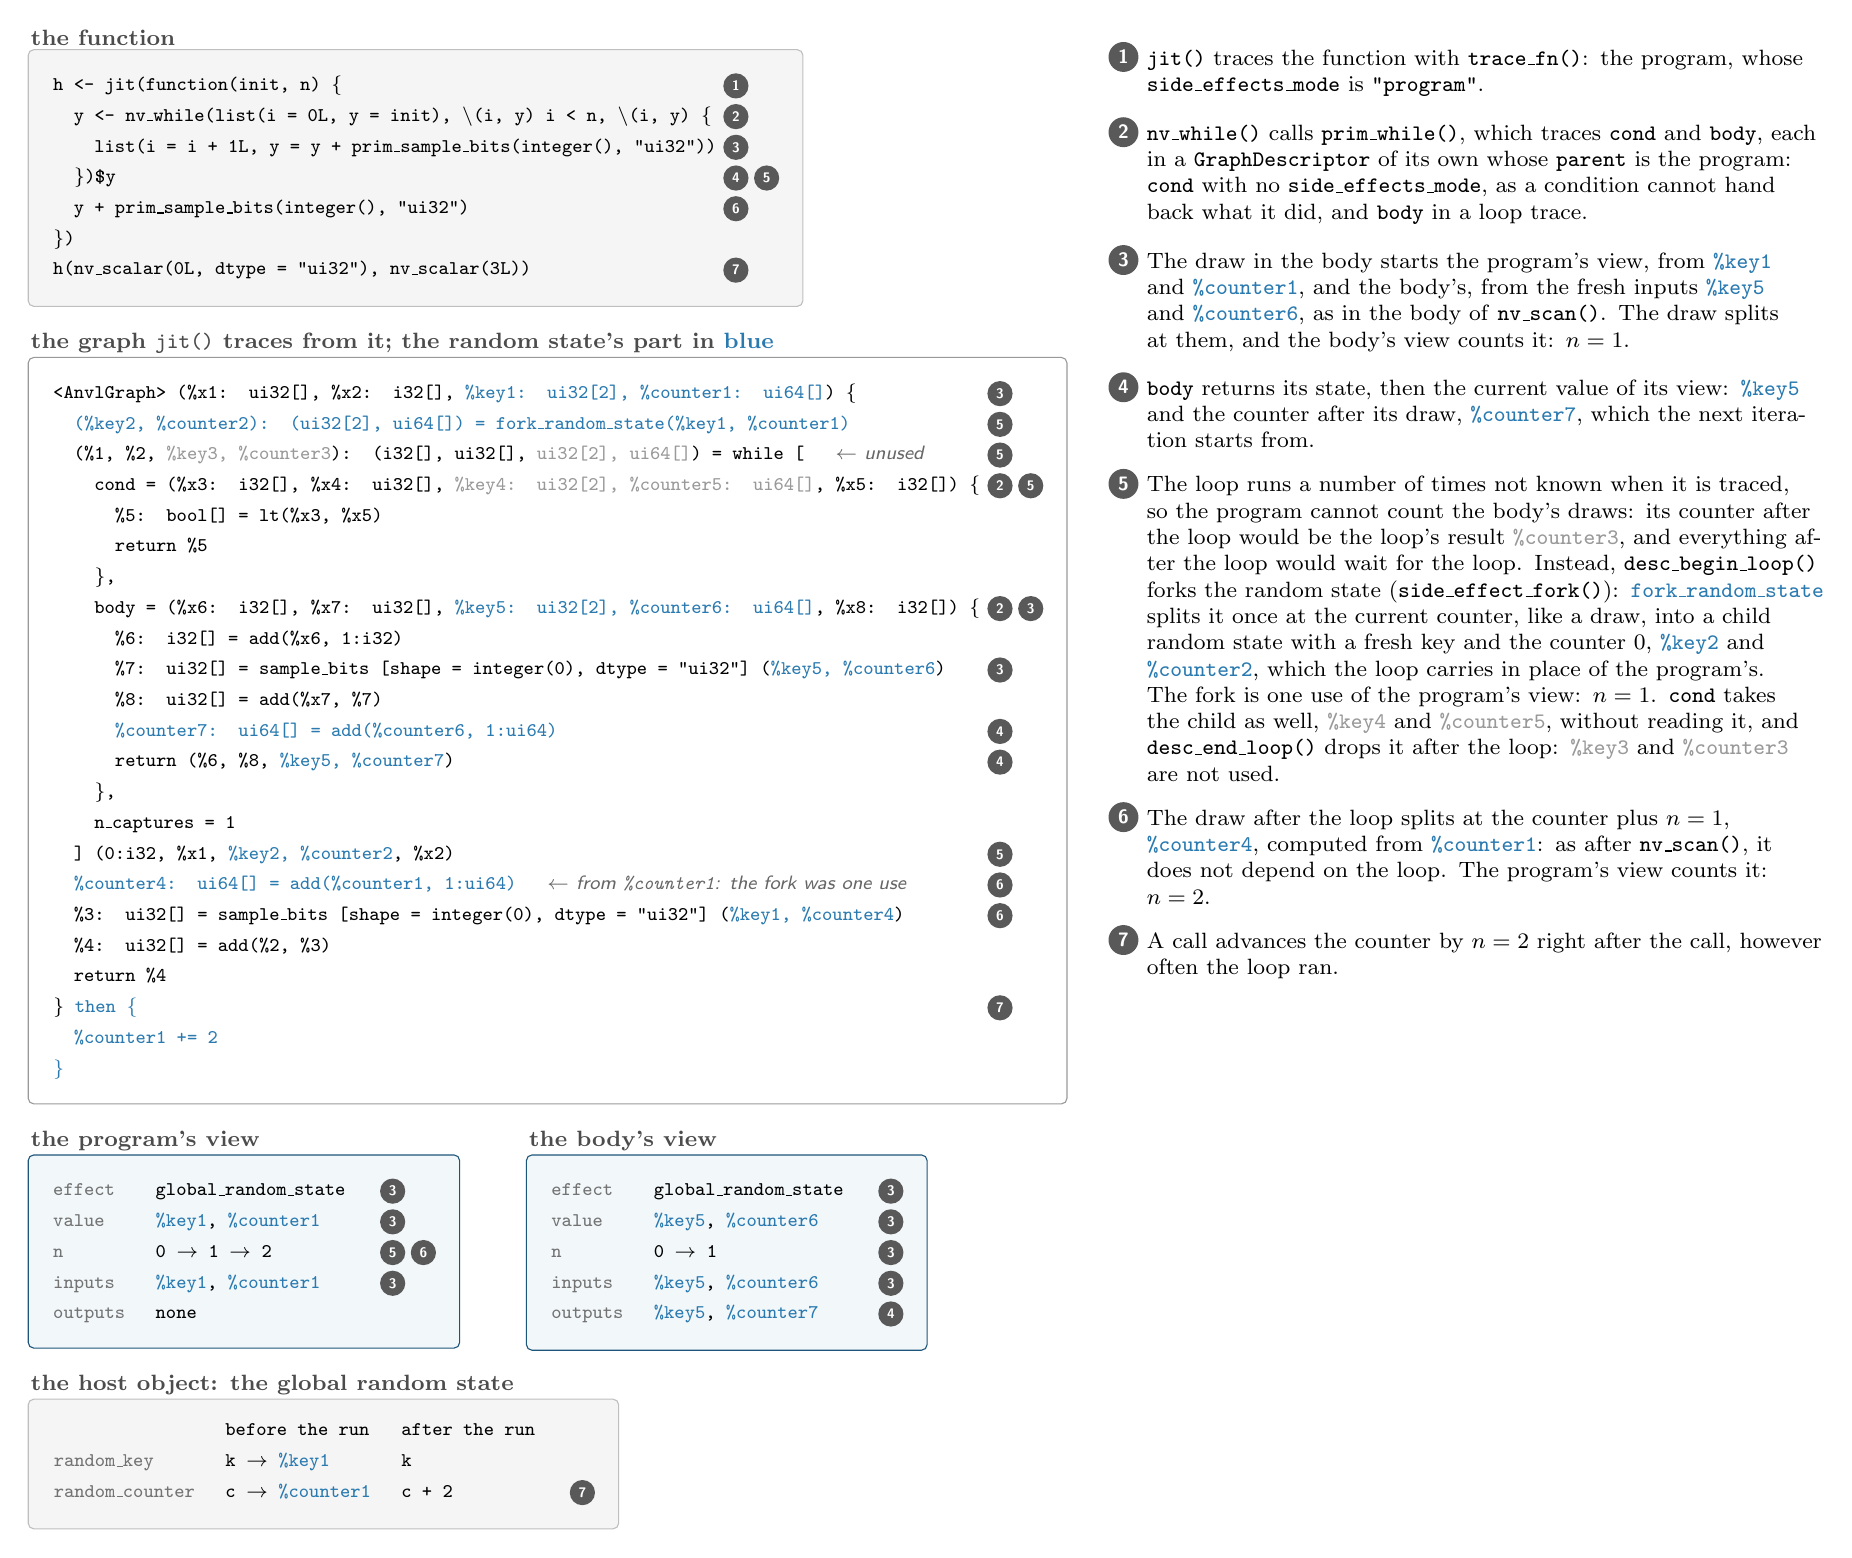
\begin{tikzpicture}
  \matrix[lines] (code) at (0, 0) {
    h <- jit(function(init, n) \{ & 1 \\
    \ \ y <- nv\_while(list(i = 0L, y = init), \textbackslash(i, y) i < n, \textbackslash(i, y) \{ & 2 \\
    \ \ \ \ list(i = i + 1L, y = y + prim\_sample\_bits(integer(), "ui32")) & 3 \\
    \ \ \})\$y & 4 & 5 \\
    \ \ y + prim\_sample\_bits(integer(), "ui32") & 6 \\
    \}) & \\
    h(nv\_scalar(0L, dtype = "ui32"), nv\_scalar(3L)) & 7 \\
  };
  \begin{scope}[on background layer]
    \node[box, draw = black!25, fill = black!4, fit = (code)] (codebox) {};
  \end{scope}
  \node[head] at (codebox.north west) {the function};

  \matrix[lines, below = 1.0 of code.south west, anchor = north west] (graph) {
    <AnvlGraph> (\%x1: ui32[], \%x2: i32[], \se{\%key1: ui32[2], \%counter1: ui64[]}) \{ & 3 \\
    \ \ \se{(\%key2, \%counter2): (ui32[2], ui64[]) = fork\_random\_state(\%key1, \%counter1)} & 5 \\
    \ \ (\%1, \%2, \unused{\%key3, \%counter3}): (i32[], ui32[], \unused{ui32[2], ui64[]}) = while [\aside{unused} & 5 \\
    \ \ \ \ cond = (\%x3: i32[], \%x4: ui32[], \unused{\%key4: ui32[2], \%counter5: ui64[]}, \%x5: i32[]) \{ & 2 & 5 \\
    \ \ \ \ \ \ \%5: bool[] = lt(\%x3, \%x5) & \\
    \ \ \ \ \ \ return \%5 & \\
    \ \ \ \ \}, & \\
    \ \ \ \ body = (\%x6: i32[], \%x7: ui32[], \se{\%key5: ui32[2], \%counter6: ui64[]}, \%x8: i32[]) \{ & 2 & 3 \\
    \ \ \ \ \ \ \%6: i32[] = add(\%x6, 1:i32) & \\
    \ \ \ \ \ \ \%7: ui32[] = sample\_bits [shape = integer(0), dtype = "ui32"] (\se{\%key5, \%counter6}) & 3 \\
    \ \ \ \ \ \ \%8: ui32[] = add(\%x7, \%7) & \\
    \ \ \ \ \ \ \se{\%counter7: ui64[] = add(\%counter6, 1:ui64)} & 4 \\
    \ \ \ \ \ \ return (\%6, \%8, \se{\%key5, \%counter7}) & 4 \\
    \ \ \ \ \}, & \\
    \ \ \ \ n\_captures = 1 & \\
    \ \ ] (0:i32, \%x1, \se{\%key2, \%counter2}, \%x2) & 5 \\
    \ \ \se{\%counter4: ui64[] = add(\%counter1, 1:ui64)}\aside{from \texttt{\%counter1}: the fork was one use} & 6 \\
    \ \ \%3: ui32[] = sample\_bits [shape = integer(0), dtype = "ui32"] (\se{\%key1, \%counter4}) & 6 \\
    \ \ \%4: ui32[] = add(\%2, \%3) & \\
    \ \ return \%4 & \\
    \} \se{then \{} & 7 \\
    \ \ \se{\%counter1 += 2} & \\
    \se{\}} & \\
  };
  \begin{scope}[on background layer]
    \node[box, draw = black!40, fit = (graph)] (graphbox) {};
  \end{scope}
  \node[head] at (graphbox.north west)
    {the graph \cd{jit()} traces from it; the random state's part in \se{blue}};

  \matrix[fields, below = 1.0 of graph.south west, anchor = north west] (pview) {
    effect &[8pt] global\_random\_state &[10pt] |[badge]| 3 \\
    value & \se{\%key1}, \se{\%counter1} & |[badge]| 3 \\
    n & 0 $\to$ 1 $\to$ 2 & |[badge]| 5 & |[badge]| 6 \\
    inputs & \se{\%key1}, \se{\%counter1} & |[badge]| 3 \\
    outputs & none \\
  };
  \begin{scope}[on background layer]
    \node[box, draw = keep!70!black, fill = keep!6, fit = (pview)] (pviewbox) {};
  \end{scope}
  \node[head] at (pviewbox.north west) {the program's view};

  \matrix[fields, anchor = north west] (bview) at ($(pview.north east) + (1.2, 0)$) {
    effect &[8pt] global\_random\_state &[10pt] |[badge]| 3 \\
    value & \se{\%key5}, \se{\%counter6} & |[badge]| 3 \\
    n & 0 $\to$ 1 & |[badge]| 3 \\
    inputs & \se{\%key5}, \se{\%counter6} & |[badge]| 3 \\
    outputs & \se{\%key5}, \se{\%counter7} & |[badge]| 4 \\
  };
  \begin{scope}[on background layer]
    \node[box, draw = keep!70!black, fill = keep!6, fit = (bview)] (bviewbox) {};
  \end{scope}
  \node[head] at (bviewbox.north west) {the body's view};

  \matrix[fields, below = 1.0 of pview.south west, anchor = north west] (host) {
    &[8pt] before the run &[8pt] after the run \\
    random\_key & k $\to$ \se{\%key1} & k \\
    random\_counter & c $\to$ \se{\%counter1} & c + 2 &[10pt] |[badge]| 7 \\
  };
  \begin{scope}[on background layer]
    \node[box, draw = black!25, fill = black!4, fit = (host)] (hostbox) {};
  \end{scope}
  \node[head] at (hostbox.north west) {the host object: the global random state};

  \coordinate (notes) at ($(codebox.north -| graphbox.east) + (1.0, 0)$);
  \note{1}{(notes)}
    {\cd{jit()} traces the function with \cd{trace\_fn()}: the program, whose
     \cd{side\_effects\_mode} is \cd{"program"}.}
  \note{2}{($(1.south west) + (0, -0.35)$)}
    {\cd{nv\_while()} calls \cd{prim\_while()}, which traces \cd{cond} and \cd{body}, each in
     a \cd{GraphDescriptor} of its own whose \cd{parent} is the program: \cd{cond} with no
     \cd{side\_effects\_mode}, as a condition cannot hand back what it did, and \cd{body} in
     a loop trace.}
  \note{3}{($(2.south west) + (0, -0.35)$)}
    {The draw in the body starts the program's view, from \se{\cd{\%key1}} and
     \se{\cd{\%counter1}}, and the body's, from the fresh inputs \se{\cd{\%key5}} and
     \se{\cd{\%counter6}}, as in the body of \cd{nv\_scan()}. The draw splits at them, and
     the body's view counts it: $n = 1$.}
  \note{4}{($(3.south west) + (0, -0.35)$)}
    {\cd{body} returns its state, then the current value of its view: \se{\cd{\%key5}} and
     the counter after its draw, \se{\cd{\%counter7}}, which the next iteration starts
     from.}
  \note{5}{($(4.south west) + (0, -0.35)$)}
    {The loop runs a number of times not known when it is traced, so the program cannot
     count the body's draws: its counter after the loop would be the loop's result
     \unused{\cd{\%counter3}}, and everything after the loop would wait for the loop.
     Instead, \cd{desc\_begin\_loop()} forks the random state (\cd{side\_effect\_fork()}):
     \se{\cd{fork\_random\_state}} splits it once at the current counter, like a draw, into
     a child random state with a fresh key and the counter 0, \se{\cd{\%key2}} and
     \se{\cd{\%counter2}}, which the loop carries in place of the program's. The fork is one
     use of the program's view: $n = 1$. \cd{cond} takes the child as well,
     \unused{\cd{\%key4}} and \unused{\cd{\%counter5}}, without reading it, and
     \cd{desc\_end\_loop()} drops it after the loop: \unused{\cd{\%key3}} and
     \unused{\cd{\%counter3}} are not used.}
  \note{6}{($(5.south west) + (0, -0.35)$)}
    {The draw after the loop splits at the counter plus $n = 1$, \se{\cd{\%counter4}},
     computed from \se{\cd{\%counter1}}: as after \cd{nv\_scan()}, it does not depend on the
     loop. The program's view counts it: $n = 2$.}
  \note{7}{($(6.south west) + (0, -0.35)$)}
    {A call advances the counter by $n = 2$ right after the call, however often the loop
     ran.}

\end{tikzpicture}
\end{document}
